L'objectif de cette semaine est de pouvoir générer un jeu de données pour la validation croisée sous weka.

\subsection{Classer les données}

Avant de poursuivre, la base de donnée à été modifiée afin d'avoir des données classées. Ceci permet de mieux se retrouver entre séquences d'acides aminées, nucléotidiques, fichier genbank, les enzymes (cox1,cox2...) ...

~\\
Chaque dossier comporte en plus des dossiers des sous taxons:

\begin{itemize}
 \item[.]Un dossier \textit{frequencies} où sera rangé les fréquences de kmers
  \item[.]un dossier \textit{data} correspondant aux données génétiques et étant constitué
  \begin{itemize}
 \item d'un dossier \textit{fasta} où sera rangé les séquences, constitué de deux sous dossiers 
  \begin{itemize}
 \item[*]\textit{aminoAcids} contenant les séquences d'acides aminés, chaque cox, cytb,...sont également rangé dans un dossier de même nom. 
 
  \item[*]\textit{nucletotides} contenant les séquences nucléotidiques, de même ici chaque cox, cytb,...sont également rangé dans un dossier de même nom. Ce dossier contient en plus un dossier \textit{genomes} contenant tous le génome complet (voir figure \ref{dossierCox}).
  
\end{itemize}
  \item d'un dossier \textit{genbank} contenant les fichiers genbank associés au taxon courant
  
\end{itemize}
\end{itemize}
~\\

\begin{figure}[H]
\begin{center}
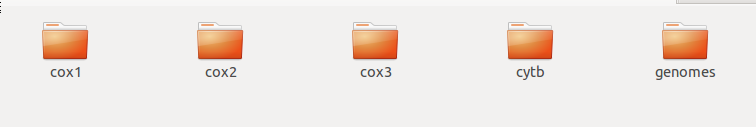
\includegraphics[scale=0.5]{./../img/dossier.png}
\caption{\label{dossierCox} Dossiers lorsqu'on se trouve dans le dossier data/fasta/nucleotides d'un taxon.}
\end{center}
\end{figure}
~\\

Cette façon de classer les données permet à l'utilisateur de pouvoir spécifier sur quelles séquences il souhaite travailler en indiquant les mots clés \textit{cox1},\textit{cox2},...ou \textit{genomes}.

\subsection{Validation croisée}

Le principe de la validation croisée, est de produire deux fichiers pour weka:
\begin{itemize}
  \item[.] Un pour l'apprentissage (80\% des séquences)
  \item[.] et un autre pour la prédiction (20\% des séquences)
\end{itemize}

Les deux fichiers de fréquences doivent avoir été construits à partir de séquences distinctes. Par exemple si $D$ est l'ensemble de nos séquences alors
on doit construire le fichier d'apprentissage à partir d'un sous ensemble $A$ et le fichier de prédiction à partir d'un sous ensemble $P$ de 
tel sorte que $A \cup P = D $ et  $ A \cap P = \emptyset $  

\subsection{Classification sous java}

Afin de pouvoir charger les données on est forcé d'utiliser le classifieur Bayes car c'est le seul à ce jour, 
permettant de charger les données petit à petit. 

\subsubsection{Quelques résultats}
En se plaçant à la racine de la base de donnée, et apprenant sur les génomes complets et avec un kmer continue de taille quatre, et essaynt de prédire des génomes complets on obtient avec le programme implémenté en java et donc avec le classifieur de Bayes 90\% d'instances correctement classées, alors qu'avec LibSVM on obtenait plus de 98\%. 


{\scriptsize \textit{Implémenter nous même notre LibSVM ?...}}
